\documentclass{article}
\usepackage{booktabs}
\usepackage{csquotes}
\usepackage{amsmath}
\usepackage{graphicx}
\usepackage{hyperref}
%\graphicspath{{C:/Users/Nikhil/Desktop/Technical Writing/security}}
\title{De-anonymization of Social Network Users}
\author{Nikhil Hiremath}
\begin{document}
\maketitle

\section*{Introduction}
`De-anonymize' is a term that keeps the mind of every cyber security analyst bugged these days.\\

Let's start understanding this in laymen terms. Think of some hoax post by a silly kid named `xyz\_patriot' on his $facebook$ wall stating \enquote{We will expose the CIA}. The hoax alarm is raised by our intelligent online web crawlers and finally they end up alerting all the security agencies throughout the world.\\

This situation is partially resolved but where our social network analysts fail is to decipher the real identity of such billions of users who are online almost every minute.\\

\section*{Previous work}
Before creating a user account every social network will ask for all the related information of the user and their email ID. But may the user `xyz\_patriot' has provided a false email false `xyz\_patriot@gmail.com' and if Google tries to track the recovery email of `xyz\_patriot' user then they may end up with another false reference. A person having bad intensions may create several such accounts in few minutes and then the person might start posting hoax message by hiding the real identity.\\

Some hackers may be interested to peek into someone's personal information (like pictures, videos), accounts (like Paypal) and may also be interested in altering-modifying or deleting online documents (like Google Docs). To fetch the real identity there were several work proposed and based on them this paper presents another way of de-anonymizing.


Inferences form previously proposed research,\\
\begin{itemize}
\item Arvind Narayanan and Shmatikov – Presented that the information from different resources can be merged, processed and used.\\
\item Griffith and Jakobsson proposed that, by co-relating the datasets from several different sources.\\
\end{itemize}

\section*{Proposed Attack Model}
The authors of this paper have presented a novel attack which deals with a practical attack idea on such anonymous social media `$S$' account holders and tracking their footprints online.\\
This idea basically revolves around the fact that the users presence on social media increases when they join the communities or group like `Manchester fan club' on $facebook$ or groups on professional network like $LinkedIn$ such as `Data Analytics and Business Intelligence Professionals Networking Group'.\\
Hence the increase in online presence at different places increases the footprints of a user online, the novel attacker exploits this fact. Since most of the times the increase in user data on social network websites, online groups and communities, the websites are prone to become more malicious.\\
So whenever a user logs into the website, his potential data is carried with the URL resulting in the user becoming vulnerable to the novel attacker's trap.\\
The attacker fetches the relevant client browser's history information and tracks the activities on the communities and posts on groups and creates a pattern of his footprints online. In other social media like, $LinkedIn$ and Google plus the user may Follow and join circles respectively.\\

The reference models proposed in background for de-anonymization attack are,\\
\begin{enumerate}
\item Social Networks

	In a social network, the relationship information established between users and group is represented by `$\Gamma(\upsilon)$'\\
\begin{equation*}	
\Gamma_g(\upsilon)=
\begin{cases}
1, & \text{if } \upsilon \text{ is a member of group g}\\
0, & \text{if } \upsilon \text{ is not a member of group g}\\
\end{cases}
\end{equation*}
Every group g has $\upsilon$ member\\
$\text{for n}\geq0$ : User $\upsilon \in {V}$ is a member of $n(v)$ groups such that \\
$\Gamma_g(\upsilon):=(\Gamma_g(\upsilon))_g \in _G $\\
And in the worst case $n=0$, the user doesn't belong to any group.\\

\item History Stealing\\
	According to the novel attack model when a victim or user $\upsilon$ visits the malicious social networking website, $S$ the browsing history is extracted by running scripts and information about visited pages id sent back to the attacker.

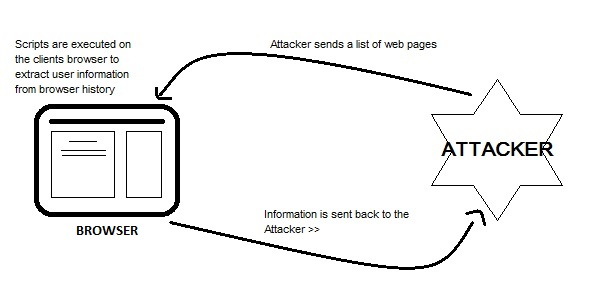
\includegraphics[scale=0.5]{History Stealing.jpg}
	
\item Attack Model

	From the browser's history $\beta(\upsilon)$ the attacker determines which ever web page $p$ the user has visited and fetch the corresponding URL $\phi(p)$.	
	
	
	Within a given time-out period $\tau$, the attacker computes $\sigma_\upsilon(\phi(p))$ to determine whether the given URL $\phi(p)$ is present in the victim $\upsilon$'s browser history $\beta_\upsilon$ or not.
	\begin{equation*}
	\sigma_\upsilon(\phi(p))=
\begin{cases}
1, & \text{if } \phi(p) \in \beta_\upsilon \text{ for the user }\upsilon \\
0, & \text{if } \phi(p) \notin \beta_\upsilon \text{ for the user }\upsilon
\end{cases}
	\end{equation*}
\end{enumerate}
\section*{Conclusion}
Thus a Basic attack would provide arbitrary user information based on the data that is retrieved specific personal details in the following way,\\
\begin{itemize}
\item On a specific link the attacker gathers relevant data.\\
\item Analyze the gathered information for identifiers like user ID and groups access.\\
\item Predict the users.\\
\end{itemize}
\section*{GITHUB Link}
\url{https://github.com/nikhilGitrepo/Security-MSCS630.git}
\end{document}